\chapter{Optical fiber}
\label{FiberOptics}

There are two fundamental types of optical fiber: single-mode and multimode. The key difference is that the multi-mode, as its name suggests, can send multiple modes simultaneously using the same physical media, while the mono-mode can only send one at a time. The modes that are regularly used for this type of link are Hermite-Gauss (HG), Laguerre-Gauss (LG) and Linearly-Polarized (LP) \cite{FiberOptics_Modes}.

Mono-mode fiber is the most used type in commercially available optical fiber links \cite{Single-Mode_Fiber_Optic}, throughout the which the fundamental Gaussian mode (HG00 = LG00) is transmitted \cite{LP_Modes}. In general, a fiber build consists mainly of an air and glass media that makes up the core, surrounded by a cladding to protect and insulate it. A model of this build can be seen in figure (\ref{fig:fiber_profile}). Keep in mind that these models can be more complicated, varying core size and cladding material depending on the fiber type, intended use and modes, as well as other variables; however, that particular discussion escapes the purposes of this paper.

\begin{figure}[htbp]
    \centering
    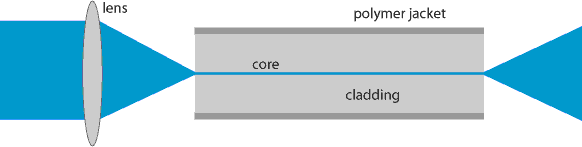
\includegraphics[width=10cm]{images/Appendices/fiber.png}
    \caption{Simple profile depicting an optical fiber build, showing its core and cladding.}
    \label{fig:fiber_profile}
\end{figure}

The simplest refractive model of an optical fiber is linear and constant for the core, and it decreases its value in the cladding. Such model is depicted in figure (\ref{fig:single-mode_fibre_refractive_index}). The refractive index by mode and type of fiber can be seen in figure (\ref{fig:multi-mode_fibre_refractive_index}).

\begin{figure}[htbp]
    \centering
    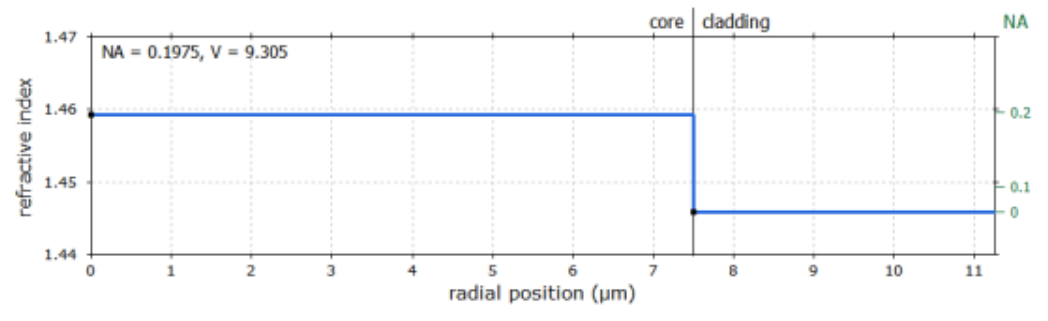
\includegraphics[width=11cm]{images/Appendices/step_index_fiber.png}
    \caption{Refractive index within a mono-mode optical fiber transmitting an LP01 mode according to its radial position and media (core or cladding) \protect\cite{Single-Mode_Fiber_Optic}.}
    \label{fig:single-mode_fibre_refractive_index}
\end{figure}

\begin{figure}[htbp]
    \centering
    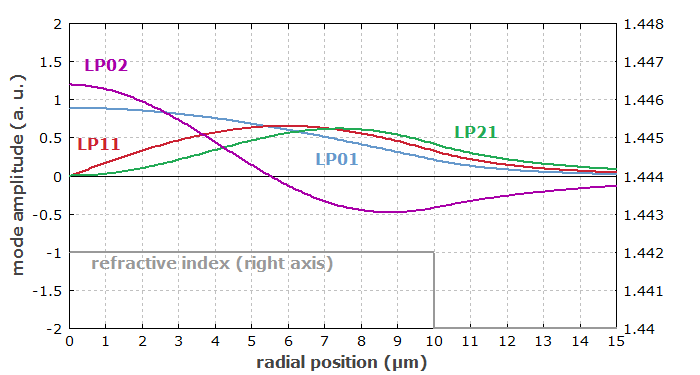
\includegraphics[width=11cm]{images/Appendices/step_index_fiber_modes.png}
    \caption{Refractive indices for different-amplitude LP modes in a multimode fiber according to their radial position. \protect\cite{FiberOptics_Refractive_Index}. Notice that all refractive indices vary around 1.444.}
    \label{fig:multi-mode_fibre_refractive_index}
\end{figure}

One of the more interesting data that can be extracted from these graphs is that optical fiber has its refractive index between $n = 1.44$ and $n = 1.46$, give or take depending on the mode and fiber type. Notice that crown glass, the type used for optical components, has a refractive index of 1.52; meanwhile, a purer form of glass known as fused silica or fused quartz, has a refractive index of 1.458 \cite{Hecht:Refractive_Index}.